\documentclass{standalone}
\usepackage{tikz}
\usetikzlibrary{patterns}
\usetikzlibrary{positioning}
\usetikzlibrary{patterns, positioning}
\usetikzlibrary{shapes.misc}
\usepackage[outline]{contour}
\contourlength{1.5pt} 
\usepackage[sfdefault]{ClearSans}

\begin{document}
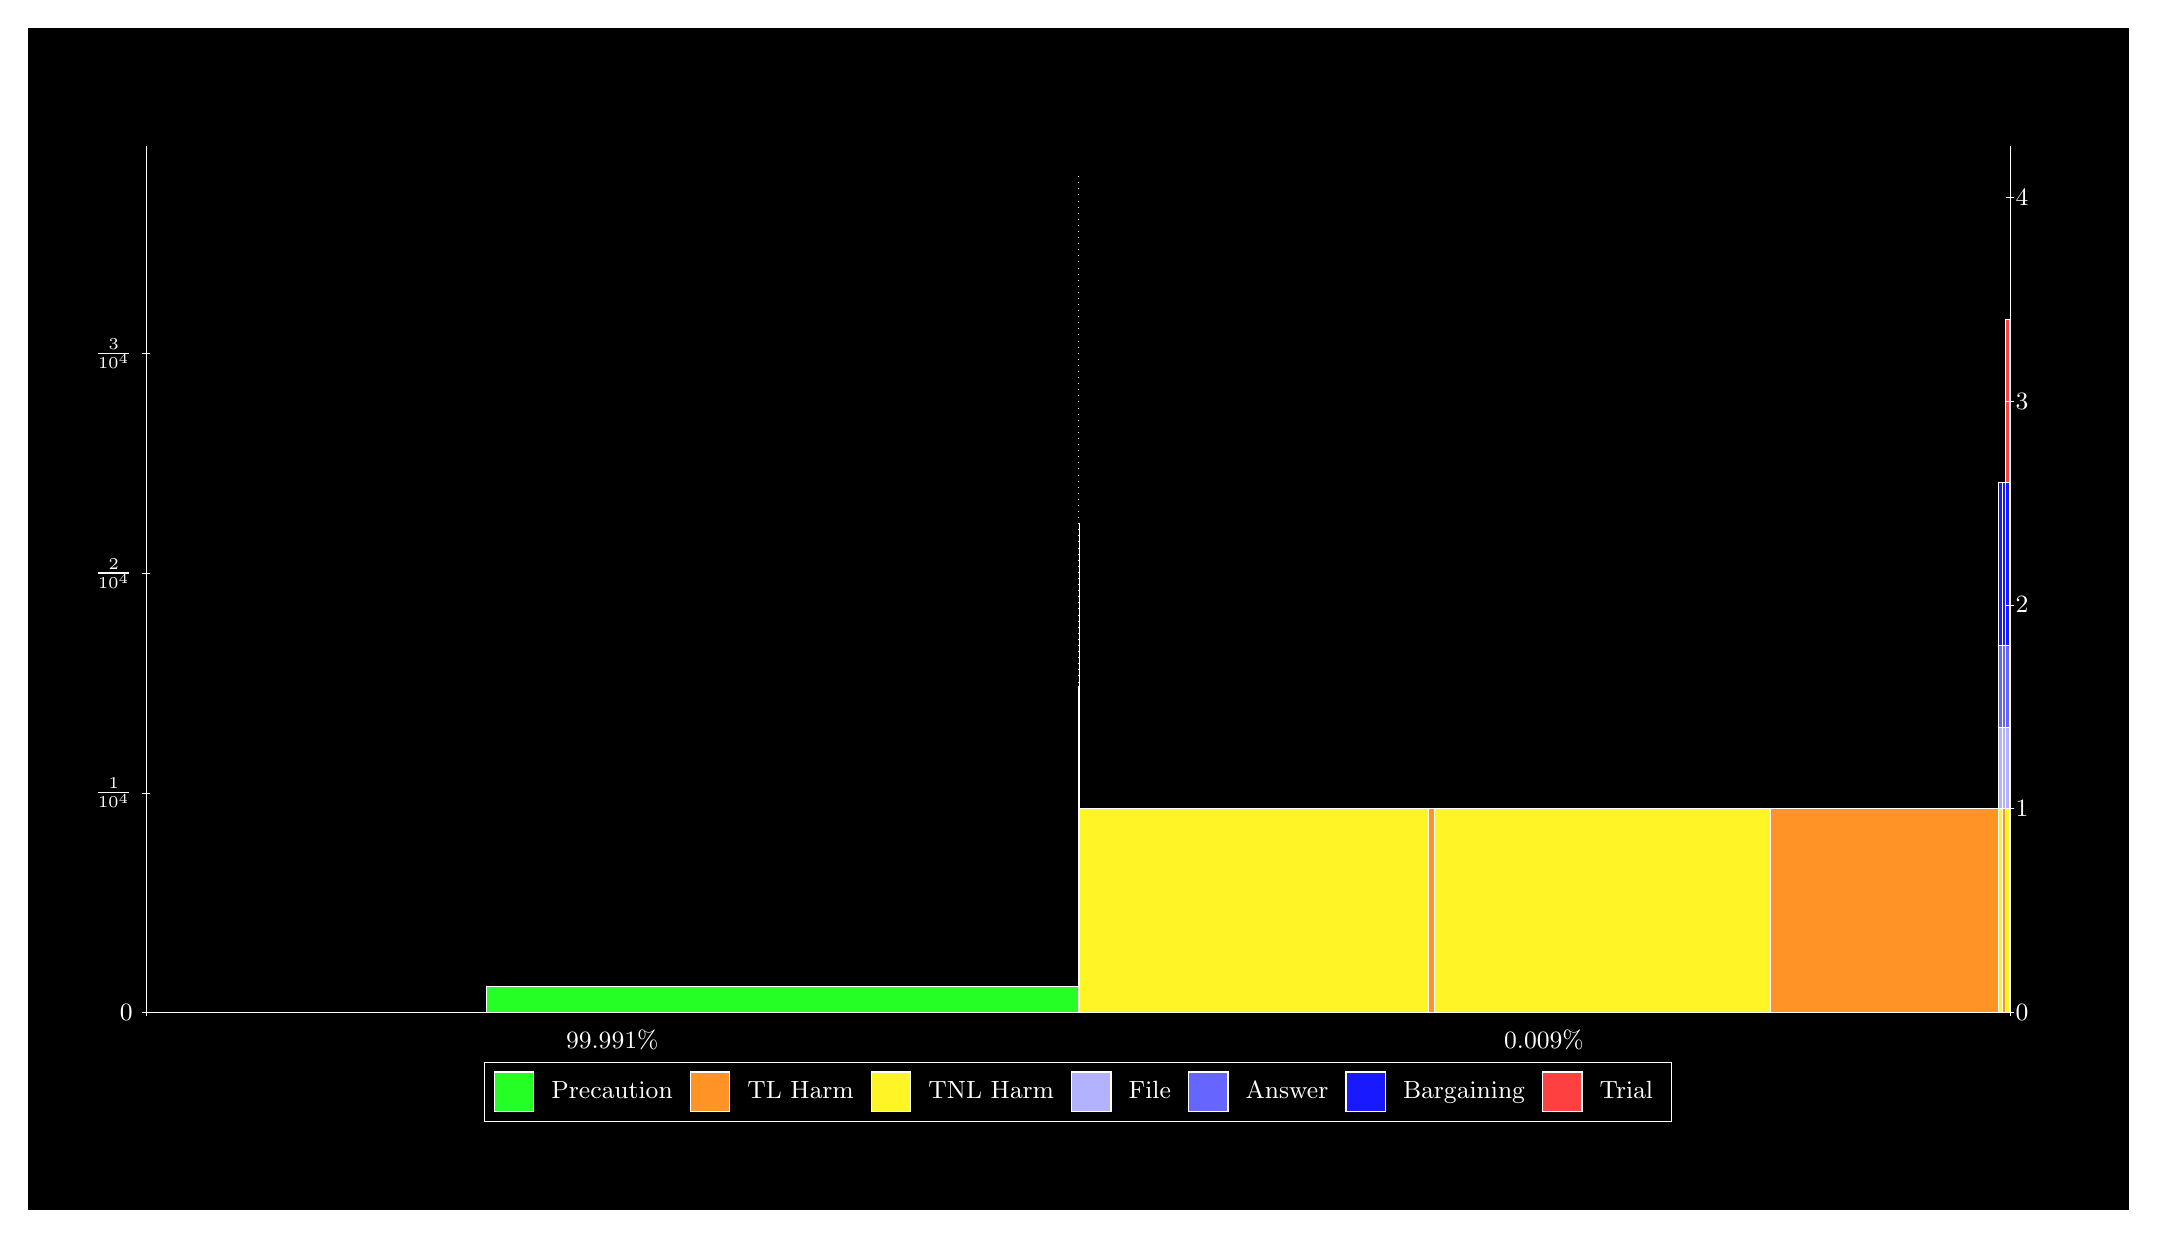
\begin{tikzpicture}
\draw[fill=black] (0,0) rectangle (26.667,15);
\draw[fill=green!85,draw=white,very thin] (5.8206,2.5) rectangle (13.333,2.8346);
\draw[fill=blue!30,draw=white,very thin] (13.333,2.5) rectangle (13.343,3.5353);
\draw[fill=blue!60,draw=white,very thin] (13.333,3.5353) rectangle (13.343,4.5706);
\draw[fill=blue!90,draw=white,very thin] (13.333,4.5706) rectangle (13.343,6.6412);
\draw[fill=blue!30,draw=white,very thin] (13.343,2.5) rectangle (13.348,3.5353);
\draw[fill=blue!60,draw=white,very thin] (13.343,3.5353) rectangle (13.348,4.5706);
\draw[fill=blue!90,draw=white,very thin] (13.343,4.5706) rectangle (13.348,6.6412);
\draw[fill=red!75,draw=white,very thin] (13.343,6.6412) rectangle (13.348,8.7118);
\draw[fill=yellow!85,draw=white,very thin] (13.348,2.5) rectangle (17.78,5.0882);
\draw[fill=orange!85,draw=white,very thin] (17.78,2.5) rectangle (17.853,5.0882);
\draw[fill=green!85,draw=white,very thin] (17.853,2.5) rectangle (22.124,2.5);
\draw[fill=yellow!85,draw=white,very thin] (17.853,2.5) rectangle (22.124,5.0883);
\draw[fill=green!85,draw=white,very thin] (22.124,2.5) rectangle (25.016,2.5);
\draw[fill=orange!85,draw=white,very thin] (22.124,2.5) rectangle (25.016,5.0883);
\draw[fill=yellow!85,draw=white,very thin] (25.016,2.5) rectangle (25.071,5.0882);
\draw[fill=blue!30,draw=white,very thin] (25.016,5.0882) rectangle (25.071,6.1235);
\draw[fill=blue!60,draw=white,very thin] (25.016,6.1235) rectangle (25.071,7.1588);
\draw[fill=blue!90,draw=white,very thin] (25.016,7.1588) rectangle (25.071,9.2294);
\draw[fill=orange!85,draw=white,very thin] (25.071,2.5) rectangle (25.114,5.0882);
\draw[fill=blue!30,draw=white,very thin] (25.071,5.0882) rectangle (25.114,6.1235);
\draw[fill=blue!60,draw=white,very thin] (25.071,6.1235) rectangle (25.114,7.1588);
\draw[fill=blue!90,draw=white,very thin] (25.071,7.1588) rectangle (25.114,9.2294);
\draw[fill=yellow!85,draw=white,very thin] (25.114,2.5) rectangle (25.156,5.0882);
\draw[fill=blue!30,draw=white,very thin] (25.114,5.0882) rectangle (25.156,6.1235);
\draw[fill=blue!60,draw=white,very thin] (25.114,6.1235) rectangle (25.156,7.1588);
\draw[fill=blue!90,draw=white,very thin] (25.114,7.1588) rectangle (25.156,9.2294);
\draw[fill=red!75,draw=white,very thin] (25.114,9.2294) rectangle (25.156,11.3);
\draw[fill=orange!85,draw=white,very thin] (25.156,2.5) rectangle (25.167,5.0882);
\draw[fill=blue!30,draw=white,very thin] (25.156,5.0882) rectangle (25.167,6.1235);
\draw[fill=blue!60,draw=white,very thin] (25.156,6.1235) rectangle (25.167,7.1588);
\draw[fill=blue!90,draw=white,very thin] (25.156,7.1588) rectangle (25.167,9.2294);
\draw[fill=red!75,draw=white,very thin] (25.156,9.2294) rectangle (25.167,11.3);
\draw[white,very thin] (1.5,2.5) -- (1.5,13.5);
\draw[white,very thin] (1.45,2.5) -- (1.55,2.5);
\node[font=\small,text=white, anchor=east] at (1.45, 2.5) {0};
\draw[white,very thin] (1.45,5.2886) -- (1.55,5.2886);
\node[font=\small,text=white, anchor=east] at (1.45, 5.2886) {$\frac{1}{10^{4}}$};
\draw[white,very thin] (1.45,8.0772) -- (1.55,8.0772);
\node[font=\small,text=white, anchor=east] at (1.45, 8.0772) {$\frac{2}{10^{4}}$};
\draw[white,very thin] (1.45,10.866) -- (1.55,10.866);
\node[font=\small,text=white, anchor=east] at (1.45, 10.866) {$\frac{3}{10^{4}}$};

\draw[white,dotted,very thin] (13.333,2.83) -- (13.333,13.17);
\draw[white,very thin] (25.167,2.5) -- (25.167,13.5);
\draw[white,very thin] (25.117,2.5) -- (25.217,2.5);
\node[font=\small,text=white, anchor=west] at (25.117, 2.5) {0};
\draw[white,very thin] (25.117,5.0882) -- (25.217,5.0882);
\node[font=\small,text=white, anchor=west] at (25.117, 5.0882) {1};
\draw[white,very thin] (25.117,7.6765) -- (25.217,7.6765);
\node[font=\small,text=white, anchor=west] at (25.117, 7.6765) {2};
\draw[white,very thin] (25.117,10.265) -- (25.217,10.265);
\node[font=\small,text=white, anchor=west] at (25.117, 10.265) {3};
\draw[white,very thin] (25.117,12.853) -- (25.217,12.853);
\node[font=\small,text=white, anchor=west] at (25.117, 12.853) {4};

\draw[white,very thin] (1.5,2.5) -- (25.167,2.5);
\draw[white,very thin] (1.5,2.45) -- (1.5,2.55);
\node[font=\small,text=white, anchor=north] at (1.5, 2.45) {};
\draw[white,very thin] (25.167,2.45) -- (25.167,2.55);
\node[font=\small,text=white, anchor=north] at (25.167, 2.45) {};

\node[font=\small,text=white,anchor=south] at (7.4167, 1.9) {99.991\%};
\node[font=\small,text=white,anchor=south] at (19.25, 1.9) {0.009\%};
\draw (13.3333,2.5) node (B) {};
\begin{scope}[align=center]
\matrix[scale=0.5,draw=white,below=0.5cm of B,nodes={draw},column sep=0.1cm]{
\node[rectangle,draw,minimum width=0.5cm,minimum height=0.5cm,fill=green!85]{}; & \node[draw=none,font=\small,text=white]{Precaution}; &
\node[rectangle,draw,minimum width=0.5cm,minimum height=0.5cm,fill=orange!85]{}; & \node[draw=none,font=\small,text=white]{TL Harm}; &
\node[rectangle,draw,minimum width=0.5cm,minimum height=0.5cm,fill=yellow!85]{}; & \node[draw=none,font=\small,text=white]{TNL Harm}; &
\node[rectangle,draw,minimum width=0.5cm,minimum height=0.5cm,fill=blue!30]{}; & \node[draw=none,font=\small,text=white]{File}; &
\node[rectangle,draw,minimum width=0.5cm,minimum height=0.5cm,fill=blue!60]{}; & \node[draw=none,font=\small,text=white]{Answer}; &
\node[rectangle,draw,minimum width=0.5cm,minimum height=0.5cm,fill=blue!90]{}; & \node[draw=none,font=\small,text=white]{Bargaining}; &
\node[rectangle,draw,minimum width=0.5cm,minimum height=0.5cm,fill=red!75]{}; & \node[draw=none,font=\small,text=white]{Trial}; \\\\
};\end{scope}

\end{tikzpicture}
\end{document}